\setcounter{chapter}{3}
\chapter{SỐ PHỨC}
\setcounter{section}{0}
\section{NHẬP MÔN SỐ PHỨC}
\subsection{TÓM TẮT LÝ THUYẾT}
\begin{tomtat}
	\subsubsection {Số phức và các khái niệm liên quan}
	\begin{boxdn}
		 Cho số phức $z=a+bi \,\left(a, b\in \mathbb{R}\right)$. Khi đó:
		\begin{itemize}
			\begin{multicols}{2}
				\item $a$ là phần thực, $b$ là phần ảo.
				\item $i$ là đơn vị ảo, $i^2=-1$.
				\item Nếu $a=0$ thì $z$ là số thuần ảo.
				\item Nếu $b=0$ thì $z$ là một số thực.
			\end{multicols}
		\end{itemize}
	\end{boxdn}
	\begin{boxdl}
	Quan hệ giữa các tập hợp số:
		\begin{itemize}
		\begin{multicols}{2}
			\item Tập số phức kí hiệu là $\mathbb{C}$.
			\item Quan hệ các tập hợp số: $\mathbb{N}\subset \mathbb{Z}\subset \mathbb{Q}\subset \mathbb{R}\subset \mathbb{C}$.
		\end{multicols}
		\end{itemize}
	\end{boxdl}
	\begin{boxdn}
		Hai số phức bằng nhau: Cho $z_1=a+bi$ và $z_2=c+di \,\, \left(a, b,c,d\in \mathbb{R}\right)$. Khi đó:
		\begin{itemize}
			\begin{multicols}{2}
				\item $z_1=z_2 \Leftrightarrow \heva{&a=c\\& b=d}$. 
				\item $z_1=0 \Leftrightarrow \heva{&a=0\\& b=0}$. 
			\end{multicols}
		\end{itemize}
	\end{boxdn}
	\begin{boxdl}
		\immini{
		Biểu diễn hình học của số phức\\
		Mỗi số phức $z=a+bi$ được biểu diễn bởi duy nhất một điểm $M(a,b)$ trên mặt phẳng tọa độ.
		}{
			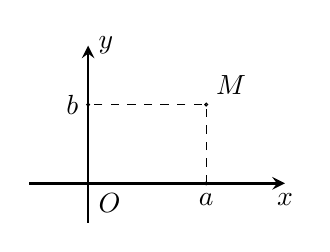
\begin{tikzpicture}[>=stealth,scale=0.5]
				\draw[->,line width = 1pt] (-1.5,0)--(0,0) node[below right]{$O$}--(5,0) node[below]{$x$};
				\draw[->,line width = 1pt] (0,-1) --(0,3.5) node[right]{$y$};
				\foreach \x in {}{
					\draw (\x,0) node[below]{$\x$} circle (1pt);
					\draw (0,\x) node[left]{$\x$} circle (1pt);
				}
				\tkzDefPoints{0/0/O,3/2/M}
				\tkzDrawPoints(O,M)
				\tkzDefPoints{0/0/A,3/2/B}
				\tkzDrawSegments[->](A,B)
				
				\draw (0,2) node[left]{$b$} circle (1pt);
				\draw (3,0) node[below]{$a$} circle (1pt);
				\draw (3,2) node[above right]{$M$} circle (1pt);
				\draw [dashed] (3,0)--(3,2)--(0,2);
			\end{tikzpicture}
		}
	\end{boxdl}
	\begin{boxdn}
		 Mô-đun số phức:
		\begin{itemize}
			\item Độ dài của véc-tơ $ \overrightarrow{OM} $ được gọi là mô-đun của số phức $ z $ và kí hiệu là $ |z| $.
			\vskip 0.15 cm
			\item Từ định nghĩa, suy ra $\boxed{|z|=\sqrt{a^2+b^2}}$ hay $ \boxed{\left|a+bi\right|=\sqrt{a^2+b^2}}$.
		\end{itemize}
		\textbf{Tính chất:}
		\begin{multicols}{2}
			\begin{itemize}
				\item $|z|\ge 0, \ \forall z\in \mathbb{C}; $ $|z|=0\Leftrightarrow z=0$. 
				\item $\left|z. z'\right|=|z|. \left|z'\right|$. 
				\item $\left|\dfrac{z}{z'}\right|=\dfrac{|z|}{\left|z'\right|}$. 
				\item $\left||z|- \left|z'\right|\right|\le \left|z\pm z'\right|\le |z|+ \left|z'\right|$. 
			\end{itemize}
		\end{multicols}
	\end{boxdn}
	\begin{boxdl}
		Số phức liên hợp: Cho số phức $ z=a+bi \,\left(a, b\in \mathbb{R}\right)$.
		\immini{
			\begin{itemize}
				\item Ta gọi $ a-bi $ là số phức liên hợp của $ z $ và kí hiệu là $ \overline z$. 
				\item Vậy, $\boxed{\overline z=a-bi}$ hay $\boxed{ \overline{a+bi}=a-bi}$
				\vskip 0.2 cm
				\item Chú ý: 
				\begin{itemize}
					\item [$\bullet$] $\boxed{z. \overline{z}={|z|}^2=a^2 + b^2}$;
					\item [$\bullet$] $z$ và $\overline{z}$ có điểm biểu diễn đối xứng nhau qua $Ox$.
				\end{itemize}	
		\end{itemize}}{
			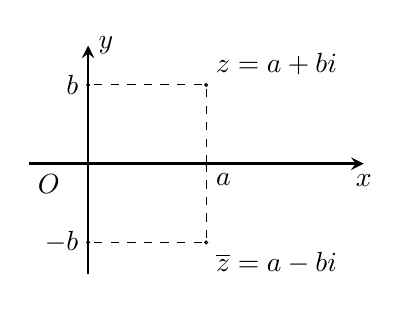
\begin{tikzpicture}[>=stealth,scale=0.5]
				\draw[->,line width = 1pt] (-1.5,0)--(-1,0) node[below]{$O$}--(7,0) node[below]{$x$};
				\draw[->,line width = 1pt] (0,-2.8) --(0,3) node[right]{$y$};
				\foreach \x in {}{
					\draw (\x,0) node[below]{$\x$} circle (1pt);
					\draw (0,\x) node[left]{$\x$} circle (1pt);
				}
				\tkzDefPoints{0/0/O,3/2/M}
				\tkzDrawPoints(O,M)
				\tkzDefPoints{0/0/A,3/2/B}
				\tkzDrawSegments[->](A,B)
				\draw (0,2) node[left]{$b$} circle (1pt);
				\draw (3,0) node[below right]{$a$} circle (1pt);
				\draw (3,2) node[above right ]{$z=a+bi$} circle (1pt);
				\draw [dashed] (3,0)--(3,2)--(0,2);
				\draw (0,-2) node[left]{$-b$} circle (1pt);
				\draw (3,-2) node[below right ]{$\overline z=a-bi$} circle (1pt);
				\draw [dashed] (3,0)--(3,-2)--(0,-2);
				\tkzDefPoints{3/-2/C}
				\tkzDrawSegments[->](A,C)
		\end{tikzpicture}}
		\end{boxdl}
	\subsubsection {Phép toán trên số phức}
\begin{boxdn} Cộng, trừ hai số phức: Ta cộng (trừ) phần thực theo phần thực, phần ảo theo phần ảo.
	\begin{itemize}
		\begin{multicols}{2}
			\item $(a+bi)+(c+di)=(a+c)+(b+d)i$.
			\item $(a+bi)-(c+di)=(a-c)+(b-d)i$.
		\end{multicols}
	\end{itemize}
\end{boxdn}
\begin{boxdl} 
	Phép nhân hai số phức: Ta nhân phân phối, tương tự nhân hai đa thức. Lưu ý: $i^2=-1$.
\end{boxdl}
\begin{boxdn}
	Phép chia hai số phức: Cho hai số phức $z_1=a+bi$ và $z_2=c+di$. Thực hiện phép chia $\dfrac{z_1}{z_2}$ , ta nhân thêm $\overline{z_2}$ ở tử và mẫu.
	\begin{align*}
		\dfrac{z_1}{z_2}=\dfrac{z_1. \overline{z_2}}{z_2. \overline{z_2}}=\dfrac{\left(a + bi\right)\left(c - di\right)}{c^2 + d^2}=\dfrac{(ac+bd)-(ad-bc)i}{c^2+d^2}=m+ni.
	\end{align*}
\end{boxdn}
\begin{boxdl} Số phức nghịch đảo của $z$ là $\dfrac{1}{z}$.
\end{boxdl}
\begin{boxdn} 
	Lũy thừa của đơn vị ảo:
	\begin{itemize}
		\begin{multicols}{2}
			\item $i^2=-1$.
			\item $i^3=-i$.
			\item $i^n=1$ nếu $n$ chia hết cho 4.
			\item $i^n=i$ nếu $n$ chia 4 dư 1.
			\item $i^n=-1$ nếu $n$ chia 4 dư 2.
			\item $i^n=-i$ nếu $n$ chia 4 dư 3.
		\end{multicols}
	\end{itemize}
\end{boxdn}	
\subsubsection {Phương trình bậc hai với hệ số thực}
\begin{boxdl}
Xét phương trình $ax^2+bx+c=0$, với $a$, $b$, $c$ $\in \mathbb{R}$ và $a\ne 0$. Đặt $\Delta =b^2 - 4ac$, khi đó:
\begin{itemize}
	\item Nếu $\Delta \ge 0$ thì phương trình có nghiệm $x_{1,2}=\dfrac{- b\pm \sqrt{\Delta}}{2a}$.
	\item Nếu $\Delta <0$ thì phương trình có nghiệm $x_{1,2}=\dfrac{- b\pm i\sqrt{\left|\Delta\right|}}{2a}$.
	\item Định lý Viet: $x_1+x_2=-\dfrac{b}{a}$ và $x_1.x_2=\dfrac{c}{a}$
\end{itemize}
\end{boxdl}
%\subsubsection {Phương trình bậc hai với hệ số phức}
%\begin{boxdl}
%Xét phương trình $ax^2+bx+c=0$, với $a$, $b$, $c$ $\in \mathbb{C}$ và $a\ne 0$. Đặt $\Delta =b^2 - 4ac=m\pm ni$.
%\begin{itemize}
%	\item Một căn bậc hai của $\Delta$ là $\Phi=\sqrt{\dfrac{|\Delta|+m}{2}}\pm i\sqrt{\dfrac{|\Delta|-m}{2}}$, với $|\Delta|=\sqrt{m^2+n^2}$.
%	\item Công thức nghiệm của phương trình là $x_{1,2}=\dfrac{- b\pm \Phi}{2a}$.
%\end{itemize}
%\end{boxdl}
\end{tomtat}

\subsection{CÁC DẠNG TOÁN THƯỜNG GẶP}
\begin{dang}{Xác định số phức bằng các phép toán}
\begin{enumerate}
	\item Thực hiện các phép toán, biến đổi số phức $z$ về dạng $A+Bi$
	\item Khi đó:
	\begin{itemize}
		\begin{multicols}{2}
			\item Phần thực là $A$; 
			\item Phần ảo là $B$;
			\item Số phức liên hợp là $\overline{z}=\overline {A+Bi}=A-Bi$;
			\item Mô - đun là $|z|=\sqrt{A^2+B^2}$
		\end{multicols}
	\end{itemize}
\end{enumerate}
\end{dang}
\setcounter{vd}{0}
\begin{vd}
Xác định phần thực và phần ảo của số phức $z$, biết:
\begin{listEX}
	\item $z=(3-2i)+(2-i)$
	\item $z=(3-2i)(2-i)$
	\item $z=\dfrac{4-2i}{2-i}$
	\item $(3+2i)z+(2-i)^2=4+i$
\end{listEX}
\loigiai{
	\begin{enumerate}[a)]
		\item $z=(3-2i)+(2-i)=5-3i$. Vậy $\heva{& a=5 \\ & b=-3}$.
		\item $z=(3-2i)(2-i)=6-2i-4i+2i^2=4-6i$. Vậy $\heva{& a=4 \\& b=-6}$.
		\item $z=\dfrac{4-2i}{2-i}=\dfrac{\left(4-2i\right)\left(2+i\right)}{4-i^2}=\dfrac{8+4i-4i-2i^2}{4+1}=2$.
		\item $(3+2i)z+(2-i)^2=4+i\Leftrightarrow z=\dfrac{4+i-\left(2-i\right)^2}{3+2i}=\dfrac{1+5i}{3+2i}=\dfrac{\left(1+5i\right)\left(3-2i\right)}{3^2-4i^2}=1+i$.
	\end{enumerate}
}
\end{vd}

\begin{vd}
Tìm phần thực và phần ảo của số phức $z = \left(\dfrac{1+i\sqrt{3}}{1+i}\right)^3$.
\loigiai{
	$z = \left(\dfrac{1+i\sqrt{3}}{1+i}\right)^3=\dfrac{\left(1+i\sqrt{3}\right)^3}{\left(1+i\right)^3}=\dfrac{1+3\sqrt{3}i+3\cdot 3i^2+3\sqrt{3}i^3}{1+3i+3i^2+i^3}=\dfrac{8}{2-2i}=\dfrac{8\left(2+2i\right)}{4-4i^2}=2+2i$.
}

\end{vd}
\begin{vd}%[2D4Y2-2]
Cho số phức $z=-\dfrac{1}{2}+\dfrac{\sqrt 3}{2}i$. Tìm số phức $w=1+z+z^2$.\dapso{$w=0$}.
\loigiai{
	$z=1-\dfrac{1}{2}+\dfrac{\sqrt{3}}{2}i+\left(-\dfrac{1}{2}+\dfrac{\sqrt{3}}{2}i\right)^2=\dfrac{1}{2}+\dfrac{\sqrt{3}}{2}i+\dfrac{3}{4}i^2-2\cdot\dfrac{1}{2}\cdot\dfrac{\sqrt{3}}{2}i+\dfrac{1}{4}=0$
}
\end{vd}

\begin{vd}%[2D4K3-2]
Tìm môđun của số phức $w=(1+z)\overline{z}$ biết rằng số phức $z$ thỏa mãn biểu thức $(3+2i)z+(2-i)^2=4+i$.\\
\dapso{$|w|=\sqrt{10}$}.
\loigiai{
	\begin{itemize}
		\item $(3+2i)z+(2-i)^2=4+i\Leftrightarrow z=\dfrac{4+i-\left(2-i\right)^2}{3+2i}=\dfrac{1+5i}{3+2i}=1+i$.
		\item $w=\left(1+1+i\right)\left(1-i\right)=3-i\Rightarrow\left|w\right|=\sqrt{3^2+(-1)^2}=\sqrt{10}$.
	\end{itemize}
}
\end{vd} 

\begin{vd}
Cho hai số phức $z_1=2+2i$ và $z_2=a+\left(a^2-6 \right)i,\,a\in\mathbb{R}$. Tìm tất cả các giá trị của $ a $ để $z_1+z_2$ là một số thực.\dapso{$a=\pm 2$}
\loigiai{
	$z_1+z_2=2+2i+a+\left(a^2-6\right)i=2+a+\left(a^2-4\right)i$.\\
	$z_1+z_2$ là số thực $\Leftrightarrow a^2-4=0\Leftrightarrow\hoac{& a=2 \\ & a=-2}$. 
}
\end{vd}

\begin{vd}
Tìm phần ảo của số phức $z=m+\left(3m+2\right)i$, ($m$ là tham số thực âm), biết rằng $\left|z\right|=2$.\dapso{$b=-\dfrac{8}{5}$}
\loigiai{
	$\left|z\right|=2\Leftrightarrow\sqrt{m^2+\left(3m+2\right)^2}=2\Leftrightarrow m^2+9m^2+12m+4=4\Leftrightarrow 10m^2+12m=0\Leftrightarrow\hoac{& m=0 \\ & m=-\dfrac{6}{5}.}$\\
	Vì $m$ là số thực âm nên chọn $m=-\dfrac{6}{5}\Rightarrow$ phần ảo của số phức $z$ là: $3\cdot\left(-\dfrac{6}{5}\right)+2=-\dfrac{8}{5}$.
}
\end{vd}

\begin{vd}%[2D4K3-2]
Tìm tất cả các giá trị thực của tham số $m$ để số phức $z=\dfrac{m+2i}{m-2i}$ có phần thực dương.\dapso{$m<-2$ hoặc $m>2$}
\loigiai{
	$z=\dfrac{m+2i}{m-2i}=\dfrac{\left(m+2i\right)\left(m+2i\right)}{m^2-4i^2}=\dfrac{m^2-4+4mi}{m^2+4}=\dfrac{m^2-4}{m^2+4}+\dfrac{4m}{m^2+4}i.$\\
	Phần thực số phức $z$ dương nên $\dfrac{m^2-4}{m^2+4}\geq 0\Leftrightarrow \hoac{& m<-2 \\ & m>2}$.
}
\end{vd}

\begin{dang}{Số phức bằng nhau}
\begin{itemize}
	\begin{multicols}{2}
		\item $a+bi=c+di \Leftrightarrow \heva{&a=c\\&b=d}$.
		\item $a+bi=0 \Leftrightarrow \heva{&a=0\\&b=0}$.
	\end{multicols}
\end{itemize}
\end{dang}
\begin{vd}%[2D4B1-1]
Tìm tất cả các giá trị thực $x$, $y$ sao cho: $x-1-yi=y+(2x-5)i$.\dapso{$x=2,y=1$}
\loigiai{
	Ta có hệ phương trình: $\heva{& x-1=y \\ & -y=2x-5}\Leftrightarrow\heva{& x-y=1 \\ & 2x+y=5}\Leftrightarrow\heva{& x=2 \\ & y=1.}$
}
\end{vd}

\begin{vd}%[2D4B3-3]
Tìm số phức $z$ thỏa mãn $(3+i)\overline{z}+(1+2i)z=3-4i$.\dapso{$z=2+5i$}
\loigiai{
	Gọi $z=x+yi$,($x,y\in \mathbb{R}$)	
	\begin{eqnarray*}
		%\everymath{\allowdisplaybreaks\displaystyle}
		& & (3+i)\overline{z}+(1+2i)z=3-4i\\
		&\Leftrightarrow& (3+i)(x-yi)+(1+2i)(x+yi)=3-4i\\
		&\Leftrightarrow& 4x-y+(3x-2y)i=3-4i\\
		&\Leftrightarrow& \heva{&4x-y=3\\&3x-2y=-4}\\
		&\Leftrightarrow& \heva{&x=2\\&y=5}\\
		&\Rightarrow& z=2+5i.
	\end{eqnarray*}
}
\end{vd}
\begin{vd}
Cho số phức $z=a + bi$, $(a, b\in \mathbb{R})$ thỏa mãn $z + 1 + 3i - |z|i=0$. Tính $S=a + 3b$.\dapso{$S=a + 3b= - 5$}
\loigiai{
	Giả sử $z=a + bi$ $(a, b\in \mathbb{R})$. Thay vào $z + 1 + 3i - |z|i=0$ ta được
	\begin{itemize}
		\item $a + bi + 1 + 3i - \sqrt{a^2 + b^2}. i=0 \Leftrightarrow (a + 1) + \left(b + 3 - \sqrt{a^2 + b^2}\right)i=0$
		\begin{align*}
			&\Leftrightarrow \heva{& a + 1=0 \\ & b + 3 - \sqrt{a^2 + b^2}=0 \\} \Leftrightarrow \heva{& a= - 1 \\ & b + 3=\sqrt{b^2 + 1} \\}\Leftrightarrow \heva{& a= - 1 \\ & \heva{& b\ge - 3 \\ 
					& b=\dfrac{- 4}{3}}} \Leftrightarrow \heva{& a= - 1 \\ & b=\dfrac{- 4}{3}};
		\end{align*}
		\item Suy ra: $S=a + 3b= - 5$.
	\end{itemize}
}
\end{vd}
%\vspace*{10cm}
\begin{dang}{Điểm biểu diễn số phức}
\immini{
	Mỗi số phức $z=a+bi$ được biểu diễn bởi duy nhất một điểm $M(a,b)$ trên mặt phẳng tọa độ. 
	\begin{itemize}
		\item [\faCheckSquareO] $|z|=OM=\sqrt{a^2+b^2}$.
\end{itemize}}{
	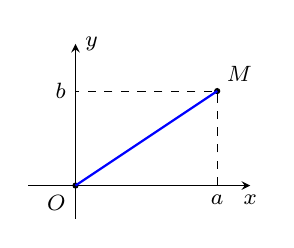
\begin{tikzpicture}[smooth,samples=300,scale=0.6,>=stealth,font=\footnotesize]
		\draw[->] (-1,0)--(3.7,0) node[below]{$x$};
		\draw[->] (0,-0.7)--(0,3) node[right]{$y$};
		\draw (0,0) node[below left]{$O$};
		\draw[fill=black] (0,0) circle(1.5pt) (3,2) circle(1.5pt);
		\draw[dashed] (3,0)node[below]{$a$}--(3,2)node[above right]{$M$}--(0,2)node[left]{$b$};
		\draw[thick,color=blue] (0,0)--(3,2);
\end{tikzpicture}}
\end{dang}
\begin{vd}
Tìm điểm biễu diễn số phức $z$, biết
\begin{listEX}
	\item $z=(2-i)^2+\dfrac{3+i}{1-i}$;
	\item $\overline{iz}=3+4i$.
\end{listEX}
\loigiai{
	\begin{enumerate}[a)]
		\item $z=\left(2-i\right)^2+\dfrac{3+i}{1-i}=3-4i+1+2i=4-3i.$\\
		Vậy điểm biểu diễn số phức $z$ là $M(4;-3)$.
	\end{enumerate}
}
\end{vd}

\begin{vd}%[2D4B1-2]
Gọi $A,B,C$ lần lượt là các điểm biểu diễn của các số phức $z_1=2$, $z_2 = 4i$, $z_3 = 2 + 4i$ trong mặt phẳng tọa độ $Oxy$. Tính diện tích tam giác $ABC$.\dapso{$S_{ABC}=4$}
\loigiai{
	\begin{itemize}
		\item $z_2-z_1=-2+4i\Rightarrow\vv{AB}=\left(-2;4\right)\Rightarrow AB=2\sqrt{5}$.
		\item $z_3-z_1=4i\Rightarrow\vv{AC}=\left(0;4\right)\Rightarrow AC=4$.
		\item $z_3-z_2=2\Rightarrow\vv{BC}=\left(2;0\right)\Rightarrow BC=2$.
		\item nửa chu vi $p=\dfrac{6+2\sqrt{5}}{2}$.
		\item Vậy diện tích tam giác $ABC$ là: $S=\sqrt{p(p-a)(p-b)(p-c)}=4.$
	\end{itemize}
}
\end{vd}

\begin{vd}%[2D4Y1-2]
\immini{Điểm $M$ trong hình vẽ bên là điểm biểu diễn của số phức $z$. Tính mô-đun của số phức $w=\dfrac{\overline{iz}(1-i)^5}{(1+i)^{10}}$.\dapso{$|w|=\dfrac{\sqrt{10}}{4}$}
}{
	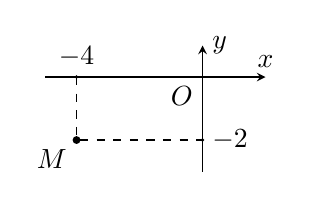
\begin{tikzpicture}[>=stealth,scale=0.4]
		\draw[->] (-5,0) --(2,0) node[above]{$x$};
		\draw[->] (0,-3) --(0,1) node[right]{$y$};
		\draw (-4,0) node[above]{$-4$} circle (1pt);
		\draw (0,-2) node[right]{$-2$} circle (1pt);
		\draw (-4,-2) node[below left]{$M$} circle (1pt);
		\draw (0,0) node[below left]{$O$};
		\draw [dashed] (-4,0)--(-4,-2)--(0,-2);
		\draw[fill] (-4,-2) circle(3pt);
	\end{tikzpicture}
}
\loigiai{
	Theo hình vẽ ta có số phức $z=-2-4i$.\\
	Thay vào biểu thức $w$ ta có:\\ $w=\dfrac{\overline{i\left(-2-4i\right)}\left(1-i\right)^5}{\left(1+i\right)^{10}}=\dfrac{\left(4+2i\right)\left(1-i\right)^2\left(1-i\right)}{\left(\left(1+i\right)^2\right)^5}=\dfrac{-24+8i}{32i}=\dfrac{1}{4}+\dfrac{3}{4}i$.\\
	Vậy modul số phức $w$ là: $\left|w\right|=\sqrt{\left(\dfrac{1}{4}\right)^2+\left(\dfrac{3}{4}\right)^2}=\dfrac{\sqrt{10}}{4}.$
}
\end{vd}

\begin{vd}%[2D4B3-4]
\immini
{
	Cho số phức $z$ thỏa mãn $|z|=\dfrac{\sqrt{2}}{2}$ và điểm $A$ trong hình vẽ bên là điểm biểu diễn của $z$. Biết rằng trong hình vẽ bên, điểm biểu diễn của số phức $w=\dfrac{1}{iz}$ là một trong bốn điểm $M, N, P, Q$. Khi đó điểm biểu diễn của số phức $w$ là
	\haicot
	{điểm $Q$}
	{điểm $M$}
	{điểm $N$}
	{\True điểm $P$}
}
{
	\begin{tikzpicture}[scale=1.3, line join=round,>=stealth,font=\footnotesize]
		\draw[->] (-1.5,0)--(1.5,0) node [below]{$x$};
		\draw[->] (0,-1.5)--(0,1.5) node [right]{$y$};
		\draw (0,0) node[below right]{$O$};
		\draw[dashed] (0.6124,0)--(0.6124,0.3535)--(0,0.3535);
		\tkzDefPoints{0/0/O,0.6124/0.3535/A, 1/0/B}
		\tkzDefPointBy[rotation=center O angle 90](A)\tkzGetPoint{M}
		\tkzDefPointBy[reflection=over O--B](M)\tkzGetPoint{N}
		\coordinate (Q) at ($(M)!-1!(O)$);
		\coordinate (P) at ($(N)!-1!(O)$);
		\tkzDrawPoints[size=2pt,fill=black](A,N,P,M,Q)
		\tkzDrawSegments(O,A O,M O,N O,P O,Q)
		\tkzLabelPoints[right](A)
		\tkzLabelPoints[left](M,N)
		\tkzLabelPoints[below](P)
		\tkzLabelPoints[above](Q)
	\end{tikzpicture}
}
\loigiai{
	Gọi $z=x+yi \left(x; y\in \mathbb{R}\right)$. Từ giả thiết, ta có $\left\{\begin{aligned}
		&x^2+y^2=\dfrac{1}{2} \\
		&x>0; y>0
	\end{aligned}\right. $. \\
	Ta có $w=\dfrac{1}{iz}=-\dfrac{i}{z}=-\dfrac{i}{x+yi}=-\dfrac{i(x-yi)}{(x+yi)(x-yi)}=-\dfrac{y+xi}{x^2+y^2}=-\,2y-2xi$. \\
	Vì $x>0, y>0$ nên điểm biểu diễn số phức $w$ có tọa độ là $\left(-\,2y;-\,2x\right)$ (đều có hoành độ và tung độ âm). Đồng thời $|w|=2\sqrt{x^2+y^2}=\sqrt{2}=2|z|$.\\
	Suy ra điểm biểu diễn của số phức $w$ nằm trong góc phần tư thứ III và cách gốc tọa độ $O$ một khoảng bằng $2OA$.\\
	Quan sát hình vẽ ta thấy có điểm $P$ thỏa mãn.
}
\end{vd}
\begin{dang}{Lũy thừa với đơn vị ảo}
\begin{enumerate}
	\item Các công thức biến đổi:
	\begin{itemize}
		\begin{multicols}{2}
			\item $i^2=-1$.
			\item $i^3=-i$.
			\item $i^n=1$ nếu $n$ chia hết cho 4.
			\item $i^n=i$ nếu $n$ chia 4 dư 1.
			\item $i^n=-1$ nếu $n$ chia 4 dư 2.
			\item $i^n=-i$ nếu $n$ chia 4 dư 3.
		\end{multicols}
	\end{itemize}
	\item Tổng $n$ số hạng đầu của một cấp số cộng:
	\begin{itemize}
		\item $S_n=\dfrac{n}{2}\left( u_1+u_n\right)$ hoặc $S_n=\dfrac{n}{2}\big[2u_1+(n-1)d\big]$, với $u_1$ là số hạng đầu, $d$ là công sai.
	\end{itemize}
	\item Tổng $n$ số hạng đầu của một cấp số nhân:
	\begin{itemize}
		\item $S_n=u_1.\dfrac{1-q^n}{1-q}$, với $u_1$ là số hạng đầu, $q$ là công bội $(q \ne 1)$.
	\end{itemize}
\end{enumerate}
\end{dang}
\begin{vd} 
Tìm số phức liên hợp của $z$, biết $z = \dfrac{i^{2009} + i^{2010} + i^{2011} + i^{2012} + i^{2013}}{i^{2014} + i^{2015} + i^{2016} + i^{2017} + i^{2018}}$.\dapso{$\overline{z}=i$}
\loigiai{
	$z=\dfrac{z^{2009}\left(1+i+i^2+i^3+i^4\right)}{i^{2014}\left(1+i+i^2+i^3+i^4\right)}=\dfrac{i^{2009}}{i^{2014}}=\dfrac{1}{i^5}=\dfrac{1}{i}=-i.$\\
	Vậy $\overline{z}=i.$
}
\end{vd}

\begin{vd}%[2D4K2-1]
Tính $S=1+i+i^2+ \cdots +i^{2017}+i^{2018}$.
\loigiai{
	Ta có $(i)^{4n}=1$, $(i)^{4n+1}=i$, $(i)^{4n+2}=-1$, $(i)^{4n+3}=-i$. Do đó\\
	$S=1+i+i^2+ \cdots +i^{2017}+i^{2018}=\dfrac{1-i^{2019}}{1-i}=\dfrac{1+i}{1-i}=i$.
}
\end{vd}

%\newpage
\NOTE
\subsection{BÀI TẬP TỰ LUYỆN}
\Opensolutionfile{ans}[ans/ansTL-CD1]
\setcounter{ex}{0}
\begin{ex}%[2D4Y1-1]
	Tìm phần thực và phần ảo của số phức liên hợp của số phức $z=1+i.$
	\choice
	{\True Phần thực là $1$, phần ảo là $-1$}
	{Phần thực là $1$, phần ảo là $-i$}
	{Phần thực là $1$, phần ảo là $1$}
	{Phần thực là $1$, phần ảo là $i$}
	\loigiai{$\bar z=1-i,$ phần thực bằng $1$, phần ảo bằng $-1$.
	}
\end{ex}
\begin{ex}%[2D4B2-1]
	Cho số phức $z_1=3+2i$, $z_2=6+5i$. Tìm số phức liên hợp của $z=6z_1+5z_2$.
	\choice
	{$\bar{z}=51+40i$}
	{$\bar{z}=51-40i$}
	{$\bar{z}=48+37i$}
	{\True $\bar{z}=48-37i$}
	\loigiai{Ta có $z=6z_1+5z_2=48+37i$ nên $\bar{z}=48-37i$.}
\end{ex}
\begin{ex}%[2D4Y1-1]
	Tính mô-đun của số phức $z$, biết rằng $z$ vừa là số thực vừa là số thuần ảo.
	\choice
	{$|z|=1$}
	{\True $|z|=0$}
	{$|z|=\sqrt{a^2+b^2}, \forall a,b\in\mathbb{R}$}
	{$|z|=i$}
	\loigiai{
		Do $z$ vừa là số thực vừa là số thuần ảo nên $z=0$.\\
		Vậy $|z|=|0|=0$.
	} 
\end{ex}
\begin{ex}%[2D4Y2-1]
	Tính mô-đun của số phức nghịch đảo của số phức $z=(1-2i)^2$.
	\choice
	{$\dfrac{1}{\sqrt{5}} $}
	{$\dfrac{1}{25} $}
	{$\sqrt{5} $}
	{\True $\dfrac{1}{5}$}
	\loigiai{
		Gọi $\omega$ là số phức nghịch đảo của số phức $z=(1-2i)^2 \Rightarrow \omega=\dfrac{1}{z}=\dfrac{-3+4i}{25}$.\\
		Vậy $|\omega|=\dfrac{1}{5}$.
	}
\end{ex}
\begin{ex}%[2D4Y1-1]
	Cho số phức $z=3+2i$. Tính $\left|z\right|$.
	\choice
	{$\left|z\right|=\sqrt 5$}
	{\True $\left|z\right|=\sqrt{13}$}
	{$\left|z\right|=5$}
	{$\left|z\right|=13$}
	\loigiai{
		Ta có $\left|z\right|=\sqrt{3^2+2^2}=\sqrt{13}$ .}
\end{ex}
\begin{ex}%[2D4B2-2]
	Cho số phức $z=2-3i$. Tính mô-đun của số phức $w=(1+i)z$.
	\choice
	{\True $|w|=\sqrt{26}$}
	{$|w|=\sqrt{37}$}
	{$|w|=5$}
	{$|w|=4$}
	\loigiai
	{
		Ta có $|w|=|(1+i)z|=|1+i|\cdot|2-3i|=\sqrt{2}\cdot\sqrt{13}=\sqrt{26}$.
	}
\end{ex}
\begin{ex}%[2D4B2-2]
	Cho số phức $z=(1-i)^2(3+2i)$. Số phức $z$ có phần ảo là
	\choice{$6$}
	{$-6i$}
	{\True $-6$}
	{$4$}
	\loigiai{
		Ta có $z=(1-i)^2(3+2i)=4-6i$. Do đó $\mathrm{Im}(z)=-6$.
	}
\end{ex}
\begin{ex}%[2D4B2-1]
	Tính $P=\left|1+\sqrt{3}i\right|^{2018}+\left|1-\sqrt{3}i\right|^{2018}$.
	\choice
	{$P=2$}
	{$P=2^{1010}$}
	{\True $P=2^{2019}$}
	{$P=4$}
	\loigiai{
		Ta có: $\left|1+\sqrt{3}i\right|=\left|1-\sqrt{3}i\right|=2$, nên $P=2^{2018}+2^{2018}=2^{2019}$.
	}
\end{ex}
\begin{ex}%[2D4B2-2]
	Nếu môđun của số phức $z$ bằng $r$ ($r>0$) thì môđun của số phức $(1-\mathrm{i})^2z$ bằng
	\choice
	{\True $2r$}
	{$4r$}
	{$r$}
	{$r\sqrt{2}$}
	\loigiai{
		Ta có $$|(1-\mathrm{i})^2z|=|(1-\mathrm{i})^2|\cdot |z|=2|z|=2r.$$
	}
\end{ex}
\begin{ex}%[2D4B1-2]
	\immini{Điểm $M$ trong hình vẽ bên là điểm biểu diễn số phức
		\haicot
		{$z=1-3i$}
		{$z=-1+3i$}
		{$z=3+i$}
		{\True $z=3-i$}
	}{
		\begin{tikzpicture}[smooth,samples=300,scale=0.8,>=stealth,font=\footnotesize]
			\draw[->] (-1,0)--(4,0) node[below]{$x$};
			\draw[->] (0,-1.5)--(0,1) node[right]{$y$};
			\draw (0,0) node[above left]{$O$};
			\draw[fill=black] (3,-1) circle(1.5pt);
			\draw[dashed] (3,-0)node[above]{$3$}--(3,-1)node[below]{$M$}--(0,-1)node[left]{$-1$};
	\end{tikzpicture}}
	\loigiai{Điểm $M(3;-1)$ là biểu diễn cho số phức $z=3-i$.}
\end{ex}
\begin{ex}
	\immini{Cho bốn số phức $z_1$, $z_2$, $z_3$ và $z_4$ có điểm biểu diễn trên mặt phẳng $Oxy$ lần lượt là $A$, $B$, $C$, $D$ như hình vẽ bên. Hỏi số phức nào có mô-đun bằng $\sqrt{13}$?
		\haicot
		{$z_1$}
		{\True $z_2$}
		{$z_3$}
		{$z_4$}
	}{
		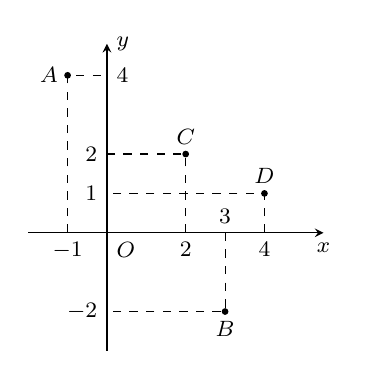
\begin{tikzpicture}[smooth,samples=300,x=0.5cm,y=0.5cm,>=stealth,font=\footnotesize]
			\draw[->] (-2,0)--(5.5,0) node[below]{$x$};
			\draw[->] (0,-3)--(0,4.8) node[right]{$y$};
			\draw (0,0) node[below right]{$O$};
			\draw[fill=black] (3,-2) circle(1pt) (4,1) circle(1pt) (-1,4) circle(1pt) (2,2) circle(1pt);
			\draw[dashed] (3,0)node[above]{$3$}--(3,-2)node[below]{$B$}--(0,-2)node[left]{$-2$}
			(-1,0)node[below]{$-1$}--(-1,4)node[left]{$A$}--(0,4)node[right]{$4$}
			(2,0)node[below]{$2$}--(2,2)node[above]{$C$}--(0,2)node[left]{$2$}
			(4,0)node[below]{$4$}--(4,1)node[above]{$D$}--(0,1)node[left]{$1$};
	\end{tikzpicture}}
	\loigiai{Điểm $B(3;-2)$ biểu diễn cho số phức $z2=3-2i$. Suy ra $|z_2|=\sqrt{3^2+(-2)^2}=\sqrt{13}$}
\end{ex}
\begin{ex}%[2D4B1-2]
	Trong mặt phẳng phức cho các điểm $A(-4;1)$, $B(1;3)$, $C(-6;0)$ lần lượt là điểm biểu diễn các số phức $z_{1}$, $z_{2}$, $z_{3}$. Trọng tâm $G$ của tam giác $ABC$ là điểm biểu diễn của số phức nào sau đây?
	\choice
	{\True $-3+\dfrac{4}{3}i$}
	{$3+\dfrac{4}{3}i$}
	{$3-\dfrac{4}{3}i$}
	{$-3-\dfrac{4}{3}i$}
	\loigiai{
		Tọa độ trọng tâm $ G $ của tam giác $ ABC $ là $ \heva{&x_{G}=-3\\ &y_{G}=\dfrac{4}{3}}\Rightarrow G\left(-3;\dfrac{4}{3} \right) $ là điểm biểu diễn của số phức $-3+\dfrac{4}{3}i$.
	}
\end{ex}
\begin{ex}%[2D4B2-2]
	Cho số phức $ z $	có điểm biểu diễn trong mặt phẳng tọa độ $ Oxy $ là điểm $ M(1;-2) $. Tính mô-đun của số phức $ w=i \bar{z}-z^2. $
	\choice
	{$ \sqrt{6} $}
	{\True $ \sqrt{26} $}
	{$ 26 $}
	{$ 6 $}
	\loigiai
	{Ta có $ z=1-2i \Rightarrow w=i(1+2i)-(1-2i)^2=i-2-(-3-4i)=1+5i. $\\
		Vậy $ \left|w\right|=\sqrt{26}. $
	}
\end{ex}
\begin{ex}%[2D4B2-2]
	Tìm hai số $x$ và $y$ thỏa mãn $\left(2x - 3yi\right) + \left(3 - i\right) = 5x - 4i$ với $i$ là đơn vị ảo.
	\choice
	{$x = - 1$; $y = - 1$}
	{$x = - 1$; $y = 1$}
	{$x = 1$; $y = - 1$}
	{\True $x = 1$; $y = 1$}
	\loigiai{ 
		Ta có 
		\begin{eqnarray*}
			& \left(2x - 3yi\right) + \left(3 - i\right) = 5x - 4i
			\Leftrightarrow 3x-3+(3y-3)i=0
			\Leftrightarrow\heva{& 3x-3=0\\& 3y-3=0}
			\Leftrightarrow\heva{& x=1\\& y=1.}
		\end{eqnarray*}
	}
\end{ex}
\begin{ex}%[2D4Y2-2]
	Tìm phần ảo của số phức $z=(a + bi)(1-2i)$ với $a,b \in \mathbb{R}$.
	\choice
	{$2a+b$}
	{$2a-b$}
	{$a+2b$}
	{\True $b-2a$}
	\loigiai{
		$z=(a + bi)(1-2i)=(a+2b)+(b-2a)i$.	
	}
\end{ex}
\begin{ex}%[2D4Y2-2]
	Cho số phức $z=a+bi$, với $a,b \in \mathbb{R}$. Phần thực của số phức $z^2$ là	
	\choice
	{$2abi$}
	{$a^2+b^2$}
	{$2ab$}
	{\True $a^2-b^2$}
	\loigiai{
		Ta có $z^2=(a+bi)^2=a^2-b^2+2abi$. Vậy phần thực của $z^2$ là $a^2-b^2$.	}
\end{ex}
\begin{ex}%[2D4Y1-2]
	Cho số phức $z=2018-2017i$. Điểm $M$ biểu diễn của số phức liên hợp của $z$ là
	\choice
	{$M(-2018;2017)$}
	{$M(2018;-2017)$}
	{$M(-2018;-2017)$}
	{\True $M(2018;2017)$}
	\loigiai{
		Số phức liên hợp của $z=2018-2017i$ là $\overline{z}=2018+2017i$. \\
		Suy ra điểm biểu diễn của $\overline{z}$ là $M(2018;2017)$.
	}
\end{ex}
\begin{ex}%[2D4B3-1]
	Tìm số phức $z$ thỏa mãn $\left(1 - 2\mathrm{i}\right)z = 3 + \mathrm{i}$.
	\choice
	{$z = 1 - \mathrm{i}$}
	{$z = 1 + \mathrm{i}$}
	{\True $z = \dfrac{1}{5} + \dfrac{7}{5}\mathrm{i}$}
	{$z = \dfrac{1}{5} - \dfrac{7}{5}\mathrm{i}$}
	\loigiai{ Ta có 
		$\left(1 - 2\mathrm{i}\right)z = 3 + \mathrm{i}\Leftrightarrow z = \dfrac{3 + \mathrm{i}}{1 - 2\mathrm{i}}\Leftrightarrow z = \dfrac{\left(3 + \mathrm{i}\right)\left(1 + 2\mathrm{i}\right)}{\left(1 - 2\mathrm{i}\right)\left(1 + 2\mathrm{i}\right)}\Leftrightarrow z = \dfrac{1}{5}\left(1 + 7\mathrm{i}\right).$
	}
\end{ex}
\begin{ex}%[2D4K3-1]
	Tìm số phức $z$ biết $z=\dfrac{3+4i}{i^{2019}}$
	\choice
	{$z=4-3i$}
	{\True $z=-4+3i$}
	{$z=3-4i$}
	{$z=3+4i$}
	\loigiai{
		Ta có: $i^{2019}=i\cdot i^{2018}=i \cdot \left(i^2\right)^{1009}=i\cdot (-1)^{1009}=-i$.\\
		KHi đó: $z=\dfrac{3+4i}{i^{2019}}=\dfrac{3+4i}{-i}=-4+3i$.	
	} 
\end{ex}
\begin{ex}%[2D4B2-1]
	Rút gọn biểu thức $P=i^{2000}+i^{2021}$.
	\choice
	{\True $P=1+i$}
	{$P=1-i$}
	{$P=-1+i$}
	{$P=-1-i$}
	\loigiai{$P=i^{2000}+i^{2021}=1+i$.}
\end{ex}
\begin{ex}%[2D4B3-2]
	Tìm phần thực và ảo của số phức $z=\dfrac{3-i}{1+i}+\dfrac{2+i}{i}$.
	\choice%4
	{Phần thực bằng $2$; phần ảo bằng $-4i$}
	{\True Phần thực bằng $2$; phần ảo bằng $-4$}
	{Phần thực bằng $2$; phần ảo bằng $4i$}
	{Phần thực bằng $-2$; phần ảo bằng $4$}
	\loigiai{
		$z=\dfrac{(3-i)i+(2+i)(1+i)}{(1+i)i}=\dfrac{2+6i}{-1+i}=2-4i.$
	}
\end{ex}
\begin{ex}%[2D4B1-1]
	Cho số phức $z= \cos \varphi + i \sin \varphi$, ($\varphi \in \mathbb{R}$). Tìm mô-đun của $z$.
	\choice
	{$|\cos \varphi | + |\sin \varphi |$}
	{\True $1$}
	{$|\cos \varphi + \sin \varphi |$}
	{$|\cos 2\varphi |$}
	\loigiai{
		Ta có $z = \cos \varphi + i \sin \varphi = 1 \left(\cos \varphi + i \sin \varphi \right)$ nên $r =1$. \\ Vậy $|z| = 1$.
	}
\end{ex}
\begin{ex}%[2D4K2-2]
	Tính môđun của số phức $z$ thoả mãn $3z\cdot \bar{z}+2017\left(z-\bar{z}\right)=48-2016i$
	\choice
	{\True $|z|=4$}
	{$|z|=\sqrt{2016}$}
	{$|z|=\sqrt{2017}$}
	{$|z|=2$}
	\loigiai{Giả sử $z=a+bi$, từ giả thiết ta có $3|z|^2=48-2016i-2b\cdot 2017i=48$ (vì $|z|^2\in \mathbb{R}$), suy ra $|z|=4$.}
\end{ex}
\begin{ex}%[2D4B2-2]
	Cho số phức $z$ thỏa mãn $2(z-1)(2-i)=(3+i)(\overline{z}+2i)$. Tìm phần thực của số phức $z^9$.
	\choice
	{$-1$}
	{$1$}
	{$-16$}
	{\True $16$}
	\loigiai{
		Đặt $z=a+bi$ với $a$, $b\in\mathbb{R}$.\\
		Khi đó 
		\begin{eqnarray*}
			&& 2(z-1)(2-i)=(3+i)(\overline{z}+2i)
			\\& \Leftrightarrow & (a-1+bi)(4-2i)=(3+i)(a-bi+2i)
			\\&\Leftrightarrow & 4a+2b-4+(-2a+4b+2)i=3a+b-2+(a-3b+6)i
			\\&\Leftrightarrow & \heva{& a+b=2\\& -3a+7b=4}\Leftrightarrow\heva{& a=1\\& b=1}
		\end{eqnarray*}
		$\Rightarrow z=1+i\Rightarrow z^9=(1+i)^9=(1+i)^8(1+i)=2^4(1+i)=16+16i$.\\
		Phần thực của $z^9$ là $16$.
	}
\end{ex}
\begin{ex}%[2D4Y1-1]
	Cho các số phức $z_1=3i$, $z_2=-1-3i$ và $z_3=m-2i$. Tập giá trị của tham số $m$ để số phức $z_3$ có mô-đun nhỏ nhất trong $3$ số phức đã cho là
	\choice
	{$\left[-\sqrt{5};\sqrt{5}\right]$}
	{\True $\left(-\sqrt{5};\sqrt{5}\right)$}
	{$\{-\sqrt{5};\sqrt{5}\}$}
	{$\left(-\infty;-\sqrt{5}\right)\cup \left(\sqrt{5};+\infty\right)$}
	\loigiai{
		Ta có $\heva{&\left|z_3\right|<\left|z_1\right|\\&\left|z_3\right|<\left|z_2\right|}\Leftrightarrow\heva{&m^2+4<9\\&m^2+4<10}\Leftrightarrow m^2<5\Leftrightarrow -\sqrt{5}<m<\sqrt{5}$.
	}
\end{ex}
\begin{ex}%[2D4B2-2]
	Tìm số thực $m$ sao cho $m^2-1+(m+1) i$ là số ảo.
	\choice
	{$m=0$}
	{$m=1$}
	{\True $m=\pm 1$}
	{$m=-1$}
	\loigiai{$m^2-1+(m+1)i$ là số ảo khi $m^2-1=0$ hay $m=\pm 1$.
	}
\end{ex}
\begin{ex}%[2D4B2-1]
	Cho $2$ số phức $z_1=1+i$, $z_2=2-mi$,$m\in\mathbb{R}$. Tìm $m$ để $z_1\cdot z_2$ là một số thuần ảo.
	\choice
	{\True $m=-2$}
	{$m=2$}
	{$m=-1$}
	{$m=1$}
	\loigiai{
		Ta có $z_1\cdot z_2 = (1+i)(2-mi) = 2+m+(2-m)i$. Để $z_1\cdot z_2$ là số thuần ảo thì $2+m=0\Leftrightarrow m=-2$.\\
		Vậy giá trị $m$ cần tìm là $m=-2$.
	}
\end{ex}
\begin{ex}%[2D4K2-1]
	Cho số phức $z=a+bi$, $(a,b\in\mathbb{R})$ thỏa $(2z-1)(1+i)-\left(\overline{z}+3i\right) (1-i)=3-7i$. Tính $P=a^2+b$.
	\choice
	{$2$}
	{$13$}
	{$7$}
	{\True $5$}
	\loigiai{
		Ta có, 
		\begin{align*}
			&(2z-1)(1+i)-\left(\overline{z}+3i\right) (1-i)=3-7i \\
			\Leftrightarrow&\quad (a-3b-4)+(3a+3b-4)i=3-7i\\
			\Leftrightarrow &\quad \heva{&a-3b=7\\&a+b=-1}\Leftrightarrow \quad \heva{&a=1\\&b=-2.}
		\end{align*}
		Khi đó, $P=a^2+b=5$.
	}
\end{ex}
\begin{ex}%[2D4B1-1]
	Biết rằng số phức $z$ có mô-đun bằng $3$ và phần ảo bằng $-3$. Tìm phần thực của số phức $z$.	
	\choice
	{$3$}
	{$6$}
	{\True $0$}
	{$\sqrt{3}$}
	\loigiai{Gọi $z=a+bi, (a,b \in \mathbb{R})$ là số phức thỏa bài toán. Khi đó $$\heva{& b=-3\\ & \sqrt{a^2+b^2}=3} \Leftrightarrow \heva{& b=-3\\ & a^2=9-(-3)^2=0} \Rightarrow a=0.$$	}
\end{ex}
\begin{ex}%[2D4B2-2]
	Cho hai số phức $z_1=m+3i$, $z_2=2-(m+1)i$, với $m\in\mathbb{R}$. Tìm các giá trị của $m$ để $w=z_1\cdot z_2$ là số thực. 
	\choice
	{$m=1$ hoặc $m=-2$}
	{$m=2$ hoặc $m=-1$}
	{\True $m=2$ hoặc $m=-3$}
	{$m=-2$ hoặc $m=-3$}
	\loigiai{Ta có $w=z_1\cdot z_2=(m+3i)\left(2-(m+1)i\right)=5m+3+\left(6-m-m^2\right)i$.\\
		Để $w$ là số thực thì $6-m-m^2=0\Leftrightarrow\hoac{&m=-3\\&m=2.}$}
\end{ex}
\begin{ex}%[2D4B2-2]
	Cho số phức $z=a+bi$ ($a$, $b$ là số thực) thỏa mãn $z+|z|-\overline{z}=5-8i$. Giá trị của biểu thức $a^2+b$ bằng
	\choice
	{$-1$}
	{\True 5}
	{$-7$}
	{12}
	\loigiai{
		Thay $|z|=\sqrt{a^2+b^2}$, $\overline{z}=a-bi$ vào phương trình đã cho, ta được
		$$a+bi+\sqrt{a^2+b^2}-a+bi=5-8i \Leftrightarrow \heva{\sqrt{a^2+b^2}=5 \\ 2b=-8} \Leftrightarrow \heva{a^2 =9 \\ b=-4}$$
		Vậy $a^2+b=5.$
	}
\end{ex}
\begin{ex}%[2D4B3-2]
	Tính tổng các giá trị của tham số thực $m$ để số phức $z=\dfrac{m-1+2(m-1)i}{1-mi}$ là số thực.
	\choice
	{$S=2\sqrt{3}$}
	{$S=15$}
	{$S=-3$}
	{\True $S=-1$}
	\loigiai{
		Ta có $z=\dfrac{m-1+2(m-1)i}{1-mi}=\dfrac{(1+mi)\left[m-1+2(m-1)i\right]}{1+m^2}=\dfrac{-2m^2+3m-1}{1+m^2}+\dfrac{m^2+m-2}{1+m^2}i$.\\
		Để $z$ là số thực thì phần ảo $\dfrac{m^2+m-2}{1+m^2}=0\Leftrightarrow m^2+m-2=0\Leftrightarrow\hoac{& m=1\\& m-2}\Rightarrow S=-1$.
	}
\end{ex}
\begin{ex}%[2D4B3-1]
	Tính tổng $S=1+i^3+i^6+ \cdots + i^{2016}$.
	\choice
	{\True $S=1$}
	{$S=-1$}
	{$S=i$}
	{$S=-i$} 
	\loigiai{
		Ta có $1,i^3,i^6, \ldots , i^{2016}$ là một cấp số nhân có $673$ số hạng với $u_1=1$ và $q = i^3$ nên 
		\begin{eqnarray*}
			S= \dfrac{1-(i^3)^{673}}{1-i^3} = \dfrac{1-i^3 \cdot (-i)^{672}}{1+i} = \dfrac{1-i^3}{1+i}=1.
		\end{eqnarray*}
	}
\end{ex}
\begin{ex}%[2D4B1-2]
	\immini
	{
		Biết tập hợp các điểm biểu diễn số phức $z=x+yi$ là nửa hình tròn tâm $O(0;0)$ bán kính $R=2$ (phần tô đậm, kể cả đường giới hạn như hình bên). Trong các khẳng định sau, khẳng định nào đúng? 
		\choice
		{$x\ge0$ và $|z|=\sqrt{2}$}
		{$y\ge0$ và $|z|=2$}
		{\True $x\ge0$ và $|z|\le2$}
		{$y\ge0$ và $|z|\le2$}
	}
	{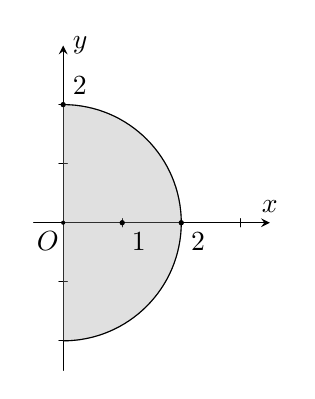
\begin{tikzpicture}[line cap=round,line join=round,x=1.0cm,y=1.0cm,>=stealth,scale=0.75]
			\draw[->] (-.5,0) --(3.5,0) node[above]{$x$};
			\draw[->] (0,-2.5) --(0,3) node[right]{$y$};
			\foreach \x in {1,2,3} 
			\draw[shift={(\x,0)},color=black] (0pt,2pt) -- (0pt,-2pt);
			\foreach \y in {-2,-1,1,2}
			\draw[shift={(0,\y)},color=black] (2pt,0pt) -- (-2pt,0pt);
			\coordinate (N) at (0,-2);
			\filldraw[fill=gray!80,opacity=0.3] (N) arc (-90:90:2cm);
			\draw (N) arc (-90:90:2cm);
			\fill (0,0) node[shift={(-130:2ex)}]{$O$} circle(1pt);
			\draw[fill] (1,0) circle (1pt) node[below right] {$1$};
			\draw[fill] (2,0) circle (1pt) node[below right] {$2$};
			\draw[fill] (0,2) circle (1pt) node[above right] {$2$};
	\end{tikzpicture}}
	\loigiai
	{
		Dựa vào hình vẽ trên ta thấy số phức $z$ có phần thực không âm và $|z|\le2$.
	}
\end{ex}
\begin{ex}%[2D4B1-3]
	\immini{Trong mặt phẳng phức, số phức thỏa mãn điều kiện nào thì có điểm biểu diễn thuộc phần gạch chéo ở hình bên (kể cả biên)?
		\choice
		{Số phức có phần thực nằm trong $(-1;1)$ và mô-đun nhỏ hơn $2$}
		{Số phức có phần thực nằm trong $[-1;1]$ và mô-đun nhỏ hơn $2$}
		{\True Số phức có phần thực nằm trong $[-1;1]$ và mô-đun không vượt quá $2$}
		{Số phức có phần thực nằm trong $(-1;1)$ và mô-đun không vượt quá $2$}}{
		\begin{tikzpicture}[scale=0.6, line join=round, line cap=round,>=stealth, font=\footnotesize]
			\draw[->] (-3,0)--(3,0) node [below]{$x$};
			\draw[->] (0,-2.7)--(0,2.7) node [left]{$y$};
			\draw (0,0) node[below left]{$O$};
			\begin{scope}
				\clip (0,0) circle (2);
				\fill[pattern=north east lines,smooth] (-1,-2)--(-1,2)--(1,2)--(1,-2)--cycle;
				\draw[->] (-1,-2)--(-1,2) (1,-2)--(1,2);
			\end{scope}
			\draw (0,0) circle(2);
			\node[below left] at (-1.9,0) {$-2$};
			\node[below right] at (2,0) {$2$};
			\node[below left] at (-0.9,0) {$-1$};
			\node[below right] at (1,0) {$1$};
	\end{tikzpicture}}
	\loigiai{
		Gọi $z=x+yi$, $(x,y \in \mathbb{R})$ có điểm biểu diễn là $M(x;y)$. Theo hình vẽ thì
		\begin{itemize}
			\item [$\bullet$] Điểm $M$ thuộc phần gạch sọc (kể cả biên) có hoành độ $x \in [-1;1]$;
			\item [$\bullet$] Điểm $M$ thuộc hình tròn tâm $O$ bán kính $r=2$ nên $|z|=OM \le 2$.
		\end{itemize}
		Vậy, phần gạch sọc (kể cả biên) ở hình bên biểu diễn số phức $z$ có phần thực nằm trong $[-1;1]$ và mô-đun không vượt quá $2$.\\
		Lưu ý: Học sinh dễ nhầm lẫn hai khái niệm "nhỏ hơn 2" và không vượt quá 2".
	}
\end{ex}
\begin{ex}
	\immini{Trong mặt phẳng tọa độ, cho điểm $M$ và $N$ lần lượt là điểm biểu diễn của số phức $z^2$ và $z^4$ (hình vẽ bên). Biết $OM=\dfrac{16}{45}\cdot ON$. Tính $|z|$.
		\haicot
		{$|z|=\dfrac{16}{45}$}
		{$|z|=\dfrac{\sqrt{5}}{3}$}
		{\True $|z|=\dfrac{3\sqrt{5}}{4}$}
		{$|z|=\dfrac{3\sqrt{3}}{4}$}
	}{
		\begin{tikzpicture}[scale=0.8, line join=round,x=0.5cm,y=0.5cm,>=stealth,font=\footnotesize]
			\draw[->] (-4,0)--(4,0) node [below]{$x$};
			\draw[->] (0,-1)--(0,8) node [left]{$y$};
			\draw (0,0) node[below right]{$O$};
			\tkzDefPoints{0/0/O,1.6875/02.25/M,-2.21484375/7.59375/N}
			\tkzDrawPoints[size=2pt,fill=black](M,N)
			\tkzLabelPoints[above right](M)
			\tkzLabelPoints[above left](N)
			\tkzDrawSegments(O,M O,N)
	\end{tikzpicture}}
	\loigiai{
		Từ $OM=\dfrac{16}{45}\cdot ON$, suy ra $\dfrac{ON}{OM}=\dfrac{45}{16}$ hay $\left| \dfrac{z^4}{z^2}\right|=\dfrac{45}{16} \Leftrightarrow |z^2|=\dfrac{45}{16} \Leftrightarrow |z|=\sqrt{\dfrac{45}{16}}=\dfrac{3\sqrt{5}}{4}$.
	}
\end{ex}
\begin{ex}%[2D4K1-1]
	Cho số phức $z$ có môđun bằng $2018$ và $w$ là số phức thỏa mãn biểu thức $\dfrac{1}{z}+\dfrac{1}{w}=\dfrac{1}{z+w}$. Môđun của số phức $w$ bằng
	\choice
	{ \True $2018$}
	{$2019$}
	{$2017$}
	{$\sqrt{2019}$}
	\loigiai{
		Từ giả thiết ta có $\dfrac{1}{z}+\dfrac{1}{w}=\dfrac{1}{z+w}\Rightarrow \dfrac{{(z+w)}^2-zw}{zw(z+w)}=0$, suy ra ${\left(z+\dfrac{1}{2}w\right)}^2={\left(-\dfrac{i\sqrt{3}w}{2}\right)}^2$.\\
		Khi đó $z=\left(-\dfrac{1}{2}-\dfrac{i\sqrt{3}}{2}\right)w$ hoặc $z=\left(-\dfrac{1}{2}+\dfrac{i\sqrt{3}}{2}\right)w\Rightarrow | w|=-\dfrac{2018}{\sqrt{\dfrac{1}{4}+\dfrac{3}{4}}}$$=2018$.}
\end{ex}
\begin{ex}%[2D4B2-2]
	Trong mặt phẳng phức, biết số phức $z$ có điểm biểu diễn nằm trong góc phần tư $(I)$. Hỏi điểm biểu diễn của số phức $w=\dfrac1{iz}$ nằm trong góc phần tư nào?
	\choice
	{$(I)$}
	{$(II)$}
	{\True $(III)$}
	{$(IV)$}
	\loigiai{Điểm biểu diễn của $iz$ chính là ảnh của điểm biểu diễn của $z$ qua phép quay tâm $O$, góc quay $90^\circ.$ Trong khi điểm biểu diễn của $\dfrac1z$ và điểm biểu diễn của $z$ khác phía đối với trục hoành và cùng phía đối với trục tung. Vậy điểm biểu diễn của $w$ thuộc góc phần tư $(III)$.
	}
\end{ex}
\begin{ex}%[2D4G2-2]
	Cho $z_1$, $z_2$ là các số phức thỏa mãn $|z_1|=|z_2|=1$ và $|z_1-2z_2|=\sqrt{6}$. Tính giá trị của biểu thức $P=|2z_1+z_2|$.
	\choice
	{\True $P=2$}
	{$P=\sqrt{3}$}
	{$P=3$}
	{$P=1$}
	\loigiai{Đặt $z_1=a_1+b_1i$; $z_2=a_2+b_2i$. Suy ra $a_1^2+b_1^2=a_2^2+b_2^2=1$.\\
		Và $|z_1-2z_2|=\sqrt{6}\Leftrightarrow a_1a_2+b_1b_2=-\dfrac{1}{4}$.\\
		Suy ra $P=|2z_1+z_2|=2$.}
\end{ex}
\begin{ex}%[2D2B4-5]
	\immini{
		Cho số phức $ z$ thỏa mãn $\left| z \right|=1$ và điểm $A$ trong hình vẽ bên là điểm biểu diễn của $ z$. Biết rằng trong hình vẽ bên, điểm biểu diễn của số phức $ w=\dfrac{1}{iz}$ là một trong bốn điểm $M,N,P,Q$. Khi đó điểm biểu diễn của số phức $w$ là
		\choice
		{Điểm $M$}
		{Điểm $N$}
		{\True Điểm $P$}
		{Điểm $Q$}}
	{	\begin{tikzpicture}[scale=0.8, line join=round,>=stealth,font=\footnotesize]
			\draw[->] (-2,0)--(2,0) node [below]{$x$};
			\draw[->] (0,-2)--(0,2) node [left]{$y$};
			\draw (0,0) node[below right]{$O$};
			\tkzDefPoints{0/0/O,0.866/0.5/A}
			\tkzDefPointBy[rotation=center O angle 120](A)\tkzGetPoint{N}
			\tkzDefPointBy[rotation=center O angle 185](A)\tkzGetPoint{P}
			\tkzDefPointBy[rotation=center O angle 100](A)\tkzGetPoint{M'}
			\tkzDefPointBy[rotation=center O angle 210](A)\tkzGetPoint{Q'}
			\coordinate (M) at ($(M')!-1!(O)$);
			\coordinate (Q) at ($(Q')!-1!(O)$);
			\tkzDrawPoints[size=2pt,fill=black](A,N,P,M,Q)
			\tkzDrawSegments(O,A O,M O,N O,P O,Q)
			\tkzLabelPoints[right](A)
			\tkzLabelPoints[left](M,N,P)
			\tkzLabelPoints[below](Q)
		\end{tikzpicture}	
	}
	\loigiai{
		Gọi $ z=x+yi\text{ }\left( x;\text{ }y\in \mathbb{R} \right)$.\\ 
		Từ giả thiết, ta có $\left\{ \begin{aligned}
			& {{x}^{2}}+{{y}^{2}}=1 \\ 
			& x>0;\text{ }y>0 \\ 
		\end{aligned} \right.$\\
		Ta có $ w=\dfrac{1}{iz}=-\dfrac{i}{z}=-\dfrac{i}{x+yi}=-\dfrac{i\left( x-yi \right)}{\left( x+yi \right)\left( x-yi \right)}=-\dfrac{y+xi}{{{x}^{2}}+{{y}^{2}}}=-\,y-xi$.\\
		Vì $ x>0,\text{ }y>0$ nên điểm biểu diễn số phức $ w$ có tọa độ là $\left( -\,y;-\,x \right)$ (đều có hoành độ và tung độ âm). Đồng thời $\left| w \right|=\sqrt{{{\left( -y \right)}^{2}}+{{\left( -x \right)}^{2}}}=1=\left| z \right|$. Suy ra điểm biểu diễn của số phức $ w$ nằm trong góc phần tư thứ III và cách gốc tọa độ $O$ một khoảng bằng $OA.$ Quan sát hình vẽ ta thấy có điểm $P$ thỏa mãn.
	}
\end{ex}
\centerline{---HẾT---}
\Closesolutionfile{ans}